\documentclass[12pt,xcolor=table,aspectratio=169]{beamer}
\usetheme{Frankfurt}
\usecolortheme{rose}
\usepackage{amsthm}
\usepackage{amsmath}
\usepackage{bbm}
\usepackage{amsfonts}
\usepackage{amssymb}
\usepackage{graphicx}
\usepackage{hyperref}
\usepackage[flushleft]{threeparttable}
\usepackage{tabularx}
\usepackage{booktabs}
\usepackage{siunitx}
\usepackage{tikz}
\usetikzlibrary{decorations.pathreplacing,angles,quotes}
%\usepackage{enumitem}% http://ctan.org/pkg/enumitem

%set up course and number

\newcommand{\ClassName}{TBD}
\newcommand{\ClassNumber}{TBD}
\newcommand{\Topic}{TBD}

% Some optional colors. Change or add as you see fit.
%---------------------------------------------------
 \definecolor{ualbertagreen}{HTML}{007C41}
\definecolor{ualbertagold}{HTML}{FFDB05}

\definecolor{calloutgrey}{HTML}{D9D9D9}


%set fonts
\setbeamerfont{subtitle}{size=\large,shape=\scshape,series=\bfseries}
\setbeamerfont{title}{size=\Large,shape=\scshape,series=\bfseries}
\setbeamerfont{author}{size=\large}
\setbeamerfont{date}{size=\large}
\setbeamerfont{caption}{size=\scriptsize}


% Some optional color adjustments to Beamer. Change as you see fit.
%------------------------------------------------------------------
\setbeamercolor{frametitle}{fg=ualbertagreen,bg=white}
\setbeamercolor{title}{fg=ualbertagreen,bg=white}
\setbeamercolor{author}{fg=ualbertagreen,bg=white}
\setbeamercolor{date}{fg=ualbertagreen,bg=white}
\setbeamercolor{local structure}{fg=ualbertagreen}
\setbeamercolor{section in toc}{fg=ualbertagreen,bg=white}
% \setbeamercolor{subsection in toc}{fg=ualbertagreen,bg=white}
\setbeamercolor{footline}{fg=ualbertagreen!50, bg=white}

% definition boxes
\setbeamercolor{block title}{bg=ualbertagreen,fg=white}
\setbeamercolor{block body}{parent=normal text,use=block title,bg=calloutgrey}
%\setbeamercolor{block body}{parent=normal text,use=block title,bg=block title.bg!30!bg}


\setbeamercolor{upper separation line head}{bg=ualbertagreen}
\setbeamercolor{lower separation line head}{bg=ualbertagold}
\setbeamercolor{middle separation line head}{bg=ualbertagold}
\setbeamercolor{frametitle}{fg=ualbertagreen,bg=white}



\setbeamercolor{section in head/foot}{bg=white,fg=ualbertagreen}
\setbeamercolor{author in head/foot}{bg=white,fg=ualbertagreen}
\setbeamercolor{date in head/foot}{bg=white,,fg=ualbertagreen}
\setbeamercolor{title in head/foot}{bg=white,fg=ualbertagreen}

\setbeamercolor{headline}{bg=white,fg=ualbertagreen}




\setbeamercolor*{middle separation line head}{bg=ualbertagreen}
\setbeamercolor*{alerted text}{fg=ualbertagreen}
\setbeamercolor*{example text}{fg=black}
\setbeamercolor*{structure}{fg=black}


\let\Tiny=\tiny



\logo{
   %\ifnum\insertpagenumber>1
   \tikz [remember picture,overlay]
    \node[yshift=.3cm,xshift=1.5cm] at (current page.south west)
        %or: (current page.center)
        {
\includegraphics[width=1in]{../images/UA-ASB-COLOUR.png}};
    %\fi
%
\includegraphics[height=0.8cm]{../images/UA-ASB-COLOUR.png}\vspace{220pt}
}


\setbeamertemplate{title page}{%
  \vbox{}
    \vspace{.5cm}% NEW
  \begingroup
    \centering
    \begin{beamercolorbox}[sep=8pt,center]{title}
      \usebeamerfont{title}\ClassNumber: \ClassName\par%
      \usebeamerfont{title}\inserttitle\par%
     \ifx\insertsubtitle\@empty%
      \else%
        \vskip0.05em%
        {\usebeamerfont{subtitle}\usebeamercolor[fg]{subtitle}\insertsubtitle\par}%
      \fi%
    \end{beamercolorbox}%
    \begin{beamercolorbox}[sep=8pt,center]{author}
      \usebeamerfont{author}\insertauthor
    \end{beamercolorbox}
    \begin{beamercolorbox}[sep=8pt,center]{institute}
      \usebeamerfont{institute}\insertinstitute
    \end{beamercolorbox}

    \vspace{0.5cm}% NEW
    \begin{beamercolorbox}[sep=8pt,center]{date}
      \usebeamerfont{date}\insertdate
    \end{beamercolorbox}\vskip0.05em

      \endgroup
  %\vfill
}


\setbeamertemplate{frametitle}{%
    \insertframetitle\par\vskip-10pt
}



\renewcommand{\ClassName}{Business Economics, Organization and Management}
\renewcommand{\ClassNumber}{BUEC 311}

\setbeamertemplate{headline}{%
\leavevmode%
 \hbox{%
    \begin{beamercolorbox}[wd=\paperwidth,ht=5ex,dp=0ex]{white}%
    \usebeamerfont{headline}\hskip6pt\ClassNumber: \inserttitle\par%
    \insertsectionnavigationhorizontal{\paperwidth}{}{\hskip0pt plus1filll}
    \end{beamercolorbox}%
  }
}

\defbeamertemplate*{footline}{my footline}{%
    \ifnum\insertpagenumber=1
        \Tiny{%
            \hfill%
		\vspace*{1pt}%
            %\insertframenumber/\inserttotalframenumber \hspace*{0.1cm}%
            \newline%
            \color{ualbertagold}{\rule{\paperwidth}{0.4mm}}\newline%
            \color{ualbertagold}{\rule{\paperwidth}{.4mm}}%
        }
  \else%
        \Tiny{%
            \hspace{.66\paperwidth}
            %\vspace{25pt}
            \insertframenumber/\inserttotalframenumber
            \newline%
            \color{ualbertagold}{\rule{\paperwidth}{0.4mm}}\newline%
            \color{ualbertagold}{\rule{\paperwidth}{.4mm}}%
        }%
    \fi%
}


\newenvironment{itemize*}%
  {\begin{itemize}%
    \setlength{\itemsep}{0pt}%
    \setlength{\parskip}{0pt}}%
  {\end{itemize}}


\title{
Oligopoly and Monopolistic Competition
}

\date{Fall 2020}

\begin{document}

\section{Outline}

\frame{
	\titlepage
}

\frame{
	\frametitle{Outline}
	\begin{enumerate}
	\item Overview
	\item[]
	\item Cartels
	\item[]
	\item Cournot Oligopoly
	\item[]
	\item Bertrand Oligopoly
	\item[]
	\item Monopolistic Competition
	\end{enumerate}
}


\section{Overview}
\frame{
	\frametitle{Outline}
	\begin{enumerate}
	\item \alert{Overview}
	\item[]
	\item Cartels
	\item[]
	\item Cournot Oligopoly
	\item[]
	\item Bertrand Oligopoly
	\item[]
	\item Monopolistic Competition
	\end{enumerate}
}

\frame{
	\frametitle{Two Additional Market Structures}
	\begin{itemize}
	\item So far, we have discussed markets with many firms (perfect competition) or one a single firm (monopoly).
	\item[]
	\item There are two additional market structures we need to consider.
		\begin{itemize}
		\item \underline{Oligopoly}: A market with few sellers and barriers to entry, so each individual firm has market power.
		\item[]
		\item \underline{Monopolistic Competition}: A market in which each firm has market power, but there is free entry in the long run.
		\end{itemize}
	\end{itemize}
}

\section{Cartels}

\frame{
	\frametitle{Outline}
	\begin{enumerate}
	\item Overview
	\item[]
	\item \alert{Cartels}
	\item[]
	\item Cournot Oligopoly
	\item[]
	\item Bertrand Oligopoly
	\item[]
	\item Monopolistic Competition
	\end{enumerate}
}

\frame{
	\frametitle{Cartels}
	\begin{itemize}
	\item Oligopolistic firms have an incentive to form a cartel in which they collude and set prices or quantities to increase profits.
		\begin{itemize}
		\item E.g. OPEC, Montreal's snowplow cartel.
		\end{itemize}
	\item[]
	\item Typically, each member of a cartel agrees to reduce its output below the level that would be individually profit maximizing.
		\begin{itemize}
		\item Idea: Increase market price, so firms in cartel earn higher profits.
			\begin{itemize}
			\item Ideally, the cartel would reduce market output to the monopoly level; this gives highest possible collective profit.
			\end{itemize}
		\item Issue: Each member of the cartel has an incentive to cheat.
		\end{itemize}
	\end{itemize}
}

\frame{
	\frametitle{Cartels}
	\begin{itemize}
	\item A cartel will form if its members believe that they can raise their profits by coordinating their actions.
	\item[]
	\item By coordinating, the cartel accounts for how output changes from each member firm affect all other members of the cartel.
	\item[]
	\item This means the aggregate profits of the cartel can exceed the combined profits of the same firms if they acted independently.
	\end{itemize}
}

\frame{
	\frametitle{Cartels}
	\begin{figure}
	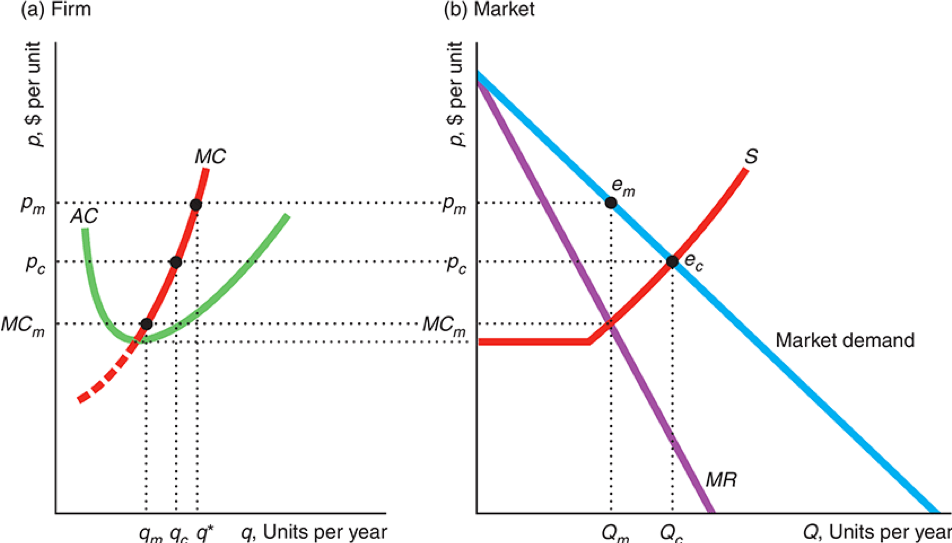
\includegraphics[scale=0.6]{../images/oligopoly/cartel.png}
	\end{figure}
}

\frame{
	\frametitle{Cartels}
	\begin{itemize}
	\item Cartels are hard to sustain in practice:
		\begin{itemize}
		\item External factors:
			\begin{itemize}
			\item Cartels are generally illegal in most developed countries. Risk of high fines/jail time may prevent collusion.
			\item Some cartels fail because they do not control enough of the market.
			\end{itemize}
		\item[]
		\item Internal factors:
			\begin{itemize}
			\item Cartel members have incentives to cheat other members of the cartel.
			\end{itemize}
		\end{itemize}
	\end{itemize}
}

\frame{
	\frametitle{Cartels}
	\begin{itemize}
	\item To sustain a cartel, members must be able to detect cheating and punish violators.
		\begin{itemize}
		\item To detect cheating:
			\begin{itemize}
			\item Some cartels give members the right to inspect each other's accounts, or divide the market by region/customer.
			\item Cartels may also turn to industry organizations to collect data on a firm's market share.
			\end{itemize}
		\item[]
		\item To enforce the cartel:
			\begin{itemize}
			\item \underline{Most-favored-customer clause}: The seller would not offer a lower price to any other current or future buyer without offering the same price decrease to the firms that signed these contracts.
			\end{itemize}
		\end{itemize}
	\end{itemize}
}

\frame{
	\frametitle{Cartels}
	\begin{itemize}
	\item Some cartels result from government policy.
		\begin{itemize}
		\item Sometimes governments help create and enforce cartels, exempting the participants from antitrust and competition laws.
		\end{itemize}
	\item[]
	\item Some cartels result from barriers to entry into a market.
		\begin{itemize}
		\item With high barriers to entry, a cartel with have few members. Fewer firms makes it easier to find cheaters and impose penalties.
		\end{itemize}
	\end{itemize}
}

\section{Cournot Oligopoly}

\frame{
	\frametitle{Outline}
	\begin{enumerate}
	\item Overview
	\item[]
	\item Cartels
	\item[]
	\item \alert{Cournot Oligopoly}
	\item[]
	\item Bertrand Oligopoly
	\item[]
	\item Monopolistic Competition
	\end{enumerate}
}

\frame{
	\frametitle{Types of Oligopoly}
	\begin{itemize}
	\item If they are not actively trying to collude and form a cartel, oligopolistic firms can compete by independently setting \underline{prices} or \underline{quantities}.
	\item[]
	\item The model we need to use to understand how oligopoly will work depends on whether firms are setting quantities or prices.
		\begin{itemize}
		\item If firms are \textbf{independently setting quantities}, we need to use the \underline{Cournot model}.
		\item If firms are \textbf{independently setting prices}, we need to use the \underline{Bertrand model}.
		\end{itemize}
	\end{itemize}
}

\frame{
	\frametitle{Cournot Oligopoly}
	\begin{itemize}
	\item The Cournot model is based on four key assumptions:
		\begin{enumerate}
		\item Few firms and no entry.
		\item Identical costs.
		\item Identical products.
		\item Firms choose output levels independently and simultaneously.
		\end{enumerate}
	\item[]
	\item Level of output is a \textit{strategic choice}.
		\begin{itemize}
		\item Firms set quantities independently, but prices adjust as needed until market clears.
			\begin{itemize}
			\item This means that firm profits are interdependent.
			\end{itemize}
		\end{itemize}
	\end{itemize}
}

\frame{
	\frametitle{Cournot Oligopoly}
	\begin{itemize}
	\item Oligopolistic firms choose output to maximize profits.
	\item[]
	\item Key departure: Firms make profit maximizing decision based on their \underline{residual demand curves}.
		\begin{itemize}
		\item The residual demand curve is the market demand that is not met by other sellers at any given price:
			\begin{align*}
			D^{r}(p) = D(p) - Q^{0}
			\end{align*}
		\end{itemize}
	\item Profit maximizing decision ($MR^{r} = MC$) yields the firm's \underline{best response}.
		\begin{itemize}
		\item Best response tells firm the profit maximizing level of output \textit{given what other sellers are producing}.
		\end{itemize}
	\end{itemize}
}

\frame{
	\frametitle{Cournot Oligopoly}
	\begin{itemize}
	\item As an example, consider competition between American Airlines and United Airlines on flights between Chicago and Los Angeles.
		\begin{itemize}
		\item This is an example of a \textit{duopoly}.
		\item Total market output: $Q = q_{A} + q_{U}$
		\end{itemize}
	\item[]
	\item For simplicity, assume that American and United face the same marginal costs.
	\item[]
	\item First step: Determine how much American will produce given United's output.
	\end{itemize}
}

\frame{
	\frametitle{Cournot Oligopoly}
	\begin{figure}
	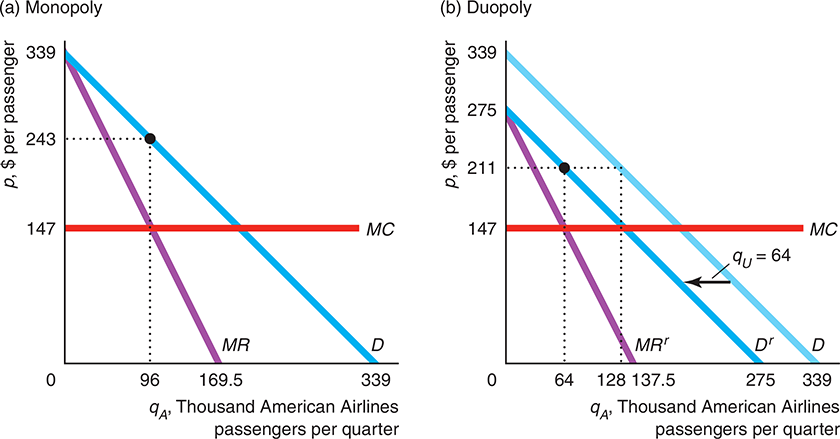
\includegraphics[scale=0.4]{../images/oligopoly/cournot.png}
	\end{figure}
}

\frame{
	\frametitle{Cournot Oligopoly}
	\begin{itemize}
	\item American repeats this exercise for every level of residual demand:
		\begin{align*}
		q_{A} = Q(p) - q_{u}
		\end{align*}
	\item This yields American's best response to any level of output from United.
	\item[]
	\item United's best response is determined in an analogous way.
	\end{itemize}
}

\frame{
	\frametitle{Cournot Oligopoly}
	\begin{figure}
	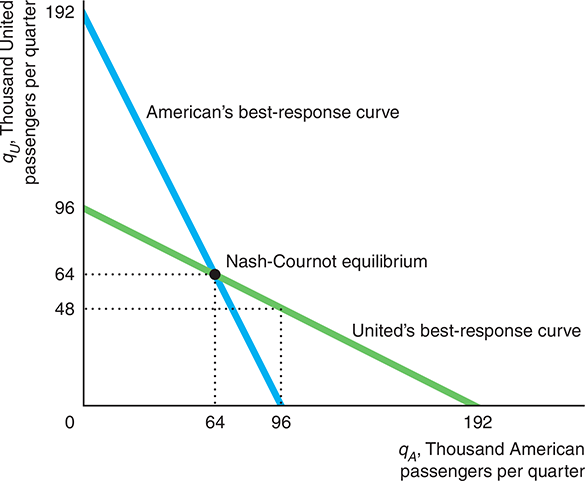
\includegraphics[scale=0.4]{../images/oligopoly/best_response.png}
	\end{figure}
}

\frame{
	\frametitle{Cournot Oligopoly}
	\begin{definition}[Nash-Cournot Equilibrium]
	A set of quantities chosen by firms such that, holding the quantities of all other firms constant, no firm can obtain a higher profit by choosing a different quantity.
	\end{definition}
	\begin{itemize}
	\item[]
	\item Equilibrium quantity must be on the best response curve for all firms.
	\end{itemize}
}

\frame{
	\frametitle{Cournot Oligopoly}
	\begin{itemize}
	\item We can also solve for the equilibrium algebraically.
	\item[]
	\item Suppose the market demand function is $Q = 339-p$ and that both companies have $MC = AC = 147$ per passenger per flight.
	\item[]
	\item The then residual demand function for American is $q_{A} = (339-p) - q_{U}$ or $p = 339 - q_{A} - q_{U}$.
	\item[]
	\item This means American's marginal revenue is given by:
		\begin{align*}
		MR^{r} = 339 - 2 q_{A} - q_{U}
		\end{align*}
	\end{itemize}
}

\frame{
	\frametitle{Cournot Oligopoly}
	\begin{itemize}
	\item American's profit maximizing choice:
		\begin{align*}
		MR^{r} &= MC\\
		339 - 2q_{A} - q_{U}& = 147
		\end{align*}
		So American's best response is:
		\begin{align*}
		q_{A} = 96 -0.5 q_{U}
		\end{align*}
	\item[]
	\item Similarly, United's best response is:
		\begin{align*}
		q_{U} = 96 -0.5 q_{A}
		\end{align*}
	\end{itemize}
}

\frame{
	\frametitle{Cournot Oligopoly}
	\begin{itemize}
	\item We can determine the Nash-Cournot equilibrium by substitution:
		\begin{align*}
		q_{A} &= 96 - 0.5 (96 - 0.5 q_{A}) =64\\
		q_{U} &= 96 - 0.5 (96 - 0.5 q_{U}) =64\\
		\end{align*}
	\item Hence, $Q = q_A + q_U = 128$, and $p=\$211$.
	\end{itemize}
}

\frame{
	\frametitle{Cournot Oligopoly}
	\begin{itemize}
	\item If two Cournot firms set output independently, the Nash-Cournot equilibrium price to consumers is lower than the monopoly price.
		\begin{itemize}
		\item It is possible to verify, with one firm, in our airline example, $Q=96$ and $p=\$243$.
		\end{itemize}
	\item[]
	\item As the number of firms increases, the equilibrium price is even lower.
		\begin{itemize}
		\item With a large enough number of firms, the Nash-Cournot equilibrium approaches the competitive outcome.
		\end{itemize}
	\end{itemize}
}

\frame{
	\frametitle{Cournot Oligopoly}
	\begin{figure}
	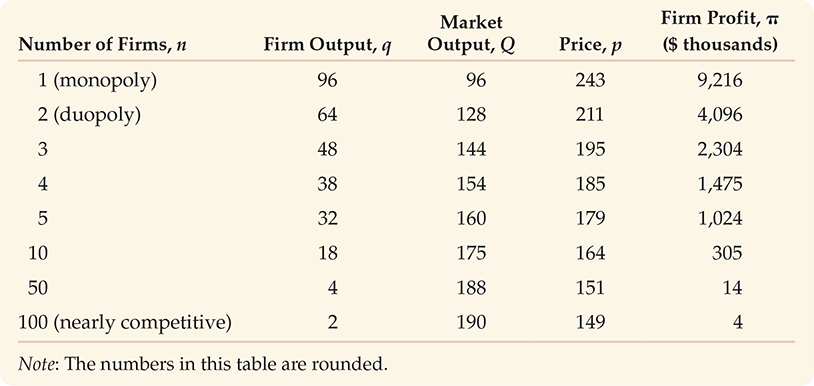
\includegraphics[scale=0.4]{../images/oligopoly/table.png}
	\end{figure}
}

\frame{
	\frametitle{Cournot Oligopoly}
	\begin{itemize}
	\item In our example, firms had the same costs and were selling the same product. In reality, firms can have different costs and/or differentiate their products.
	\item[]
	\item In the Cournot model, a change in costs shifts a firm's best response function.
		\begin{itemize}
		\item Recall: For a profit maximizing firm, $MR=MC$, so a change in cost changes what level of output is profitable given what other firms are doing.
		\end{itemize}
	\item[]
	\item As an example, suppose that United's $MC$ falls from \$147 to \$99.
	\end{itemize}
}

\frame{
	\frametitle{Cournot Oligopoly}
	\begin{figure}
	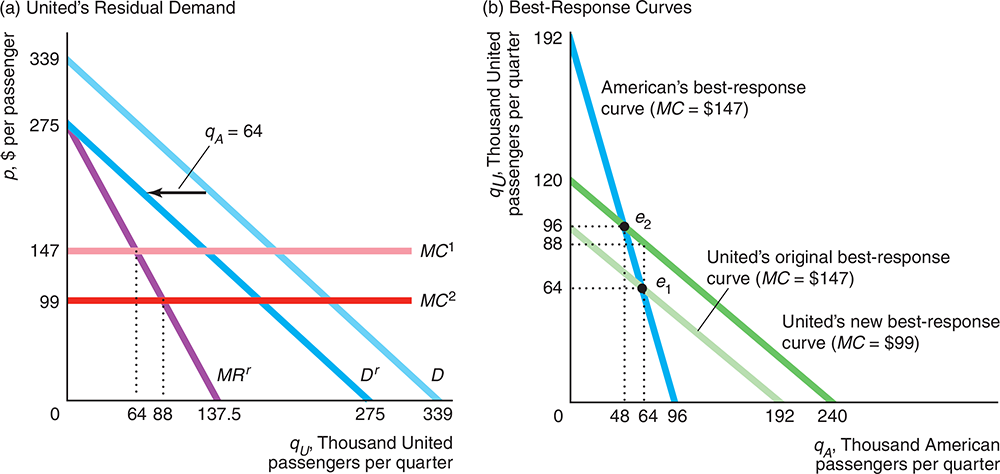
\includegraphics[scale=0.4]{../images/oligopoly/mc_drop.png}
	\end{figure}
}

\frame{
	\frametitle{Cournot Oligopoly}
	\begin{itemize}
	\item If an oligopolistic firm can differentiate its products from its rivals, it can shift its demand curve to the right and make it less elastic.
	\item[]
	\item The less elastic the demand curve, the more the firm can charge because consumers are willing to pay more for a product that ``seems'' superior.
	\item[]
	\item Although differentiation leads to higher prices, which harms consumers, differentiation can be desirable in its own right.
		\begin{itemize}
		\item Consumers value having a choice, and some may prefer new brands to existing ones.
		\end{itemize}
	\item[]
	\item If consumers think products differ, then Cournot quantities and prices may differ across firms.
		\begin{itemize}
		\item Each firm faces a different inverse demand function and hence, charges a different price.
		\end{itemize}
	\end{itemize}
}

\frame{
	\frametitle{Cournot Oligopoly}
	\begin{itemize}
	\item Oligopolistic firms may desire to merge to increase profit.
	\item[]
	\item In general there are two types of mergers:
		\begin{enumerate}
		\item \underline{Vertical mergers} that may lower cost with more efficient supply chain organization.
		\item \underline{Horizontal mergers} that may increase market power and reduce competition.
		\end{enumerate}
	\item[]
	\item Mergers designed to reduce competition are rarely profitable unless accompanied by a cost reduction.
	\end{itemize}
}

\section{Bertrand Oligopoly}

\frame{
	\frametitle{Outline}
	\begin{enumerate}
	\item Overview
	\item[]
	\item Cartels
	\item[]
	\item Cournot Oligopoly
	\item[]
	\item \alert{Bertrand Oligopoly}
	\item[]
	\item Monopolistic Competition
	\end{enumerate}
}

\frame{
	\frametitle{Bertrand Oligopoly}
	\begin{itemize}
	\item In the Bertrand model, \textbf{prices are the strategic choice}.
		\begin{itemize}
		\item Firms set prices and then consumers decide how many units to buy.
		\end{itemize}
	\item[]
	\item Firms must  account for the pricing decisions of all other firms in the market.
		\begin{itemize}
		\item E.g. Duopoly
			\begin{itemize}
			\item Firm 1's best response curve comes from answering ``What price should we (Firm 1) set if Firm 2 sets a price of $p_{2}=x$?'' for all possible values of $x$.
			\item Firm 2's best response curve comes from answering ``What price should we (Firm 2) set if Firm 1 sets a price of $p_{1}=y$?'' for all possible values of $y$.				\end{itemize}
		\end{itemize}
	\end{itemize}
}

\frame{
	\frametitle{Bertrand Oligopoly}
	\begin{definition}[Nash-Bertrand Equilibrium]
	The set of prices such that no firm can obtain a higher profit by choosing a different price if the other firms continue to charge these prices.
	\end{definition}
	\begin{itemize}
	\item[]
	\item Nash-Bertrand equilibrium differs from the Nash-Cournot equilibrium; with Bertrand, firms only earn positive profits if they produce differentiated products.
	\end{itemize}
}

\frame{
	\frametitle{Bertrand Oligopoly}
	\begin{itemize}
	\item As an example, consider a price-setting oligopoly where firms have identical costs and produce identical products.
	\item[]
	\item Suppose there are two firms (Firm 1 and Firm 2) that produce identical products, and have identical costs so $MC=AC=\$5$.
	\item[]
	\item What price should each firm charge?
	\end{itemize}
}

\frame{
	\frametitle{Bertrand Oligopoly}
	\begin{figure}
	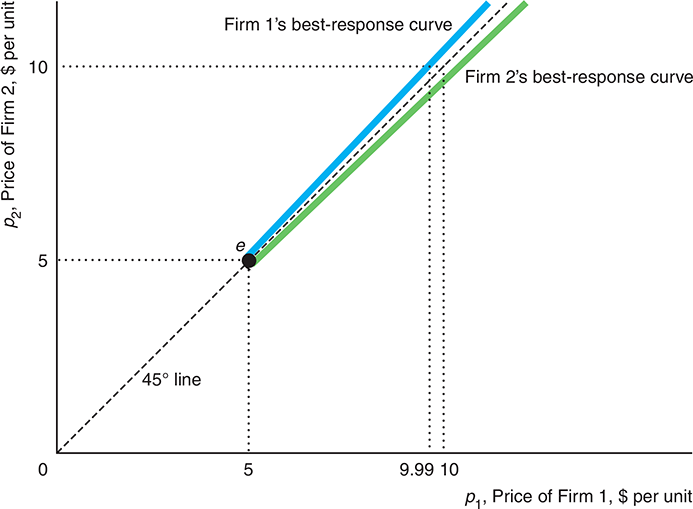
\includegraphics[scale=0.4]{../images/oligopoly/identical.png}
	\end{figure}
}

\frame{
	\frametitle{Bertrand Oligopoly}
	\begin{itemize}
	\item When firms produce identical products, the Nash-Bertrand Equilibrium outcome is the same equilibrium as perfect competition.
	\item[]
	\item This seems implausible for two reasons:
		\begin{enumerate}
		\item In a market with few firms, why would firms compete so vigorously that they earn no profit?
		\item Equilibrium depends only on costs; it is insensitive to demand conditions or the number of firms.
		\end{enumerate}
	\item[]
	\item \underline{Implication}: Nash-Cournot model is better suited for understanding markets with identical products.
	\end{itemize}
}

\frame{
	\frametitle{Bertrand Oligopoly}
	\begin{itemize}
	\item The Bertrand model is better suited for understanding markets featuring differentiated products.
	\item[]
	\item E.g. Coke and Pepsi
		\begin{itemize}
		\item Two firms with nearly identical costs:
			\begin{align*}
			MC = AC = \$5
			\end{align*}
		\item Products are differentiated, so some consumers prefer one to the other regardless of price.
			\begin{itemize}
			\item This means neither firm has to exactly match a price cut by its rival.
			\end{itemize}
		\end{itemize}
	\end{itemize}
}

\frame{
	\frametitle{Bertrand Oligopoly}
	\begin{figure}
	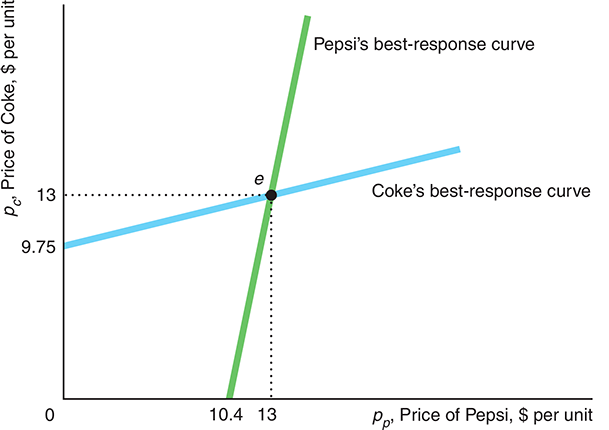
\includegraphics[scale=0.4]{../images/oligopoly/different.png}
	\end{figure}
}

\section{Monopolistic Competition}

\frame{
	\frametitle{Outline}
	\begin{enumerate}
	\item Overview
	\item[]
	\item Cartels
	\item[]
	\item Cournot Oligopoly
	\item[]
	\item Bertrand Oligopoly
	\item[]
	\item \alert{Monopolistic Competition}
	\end{enumerate}
}

\frame{
	\frametitle{Monopolistic Competition}
	\begin{itemize}
	\item Final market structure: \underline{Monopolistic Competition}
		\begin{itemize}
		\item Features the price setting characteristics of monopoly and oligopoly and the free entry of perfect competition.
			\begin{itemize}
			\item Firms face downward sloping demand curves, and have market power.
			\item Firms may earn zero profit in the long run due to free entry.
			\end{itemize}
		\end{itemize}
	\item[]
	\item Demand may be downward sloping for two reasons:	
		\begin{enumerate}
		\item Market demand may be limited so there is only room in the market for a few firms; each firm faces a residual demand curve that is downward sloping.
			\begin{itemize}
			\item E.g. A market may only be large enough to support a few service providers (barbers/plumbers/etc).
			\end{itemize}
		\item Firms produce differentiated products. Each firm can retain those customers who like product more even if its prices is above that of rivals.
			\begin{itemize}
			\item E.g. Food trucks.
			\end{itemize}
		\end{enumerate}
	\end{itemize}
}

\frame{
	\frametitle{Monopolistic Competition}
	\begin{figure}
	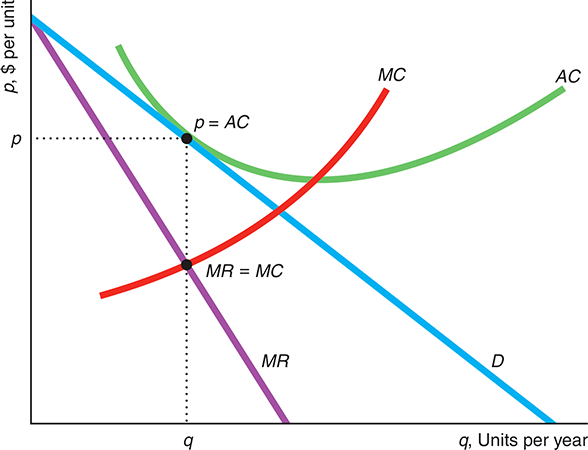
\includegraphics[scale=0.4]{../images/oligopoly/mon_comp.png}
	\end{figure}
}

\frame{
	\frametitle{Monopolistic Competition}
	\begin{itemize}
	\item If all firms in a monopolistically competitive market produce identical products and have identical costs, each firm earns \textit{zero economic profit in the long run}.
	\item[]
	\item If firms have different cost functions or produce differentiated products, then firms will likely differ in their long run profitability.
		\begin{itemize}
		\item Low-cost firms, or firms with superior products may earn positive economic profit in the long run.
		\end{itemize}
	\end{itemize}
}

\frame{
	\frametitle{Takeaways}
	\begin{enumerate}
	\item Oligopolistic firms have an incentive to collude and form a cartel.
	\item[]
	\item In oligopolies, firm profits are interdependent. Profitability depends on differences in cost and product differentiation.
	\item[]
	\item In monopolistically competitive markets, profitability also depends on differences in cost and product differentiation. If firms produce identical goods with identical costs, they all earn zero economic profit in the long run.
	\end{enumerate}
}


\end{document}

